\chapter{Implementation}
% This chapter should describe what was actually produced: the programs which were written, the hardware which was built or the theory which was developed. Any design strategies that looked ahead to the testing stage might profitably be referred to (the professional approach again).
% Descriptions of programs may include fragments of high-level code but large chunks of code are usually best left to appendices or omitted altogether. Analogous advice applies to circuit diagrams.
% Draw attention to the parts of the work which are not your own. The Implementation Chapter should include a section labelled ”Repository Overview”. The repository overview should be around one page in length and should describe the high-level structure of the source code found in your source code Repository. It should describe whether the code was written from scratch or if it built on an existing project or tutorial. Making effective use of powerful tools and pre-existing code is often laudable, and will count to your credit if properly reported.
% It should not be necessary to give a day-by-day account of the progress of the work but major milestones may sometimes be highlighted with advantage.

%  ~4,500 words

% Tangent works better than correlation or partial correlation.
\section{Overview}
\flushbottom
\begin{figure}[]
    \centering
    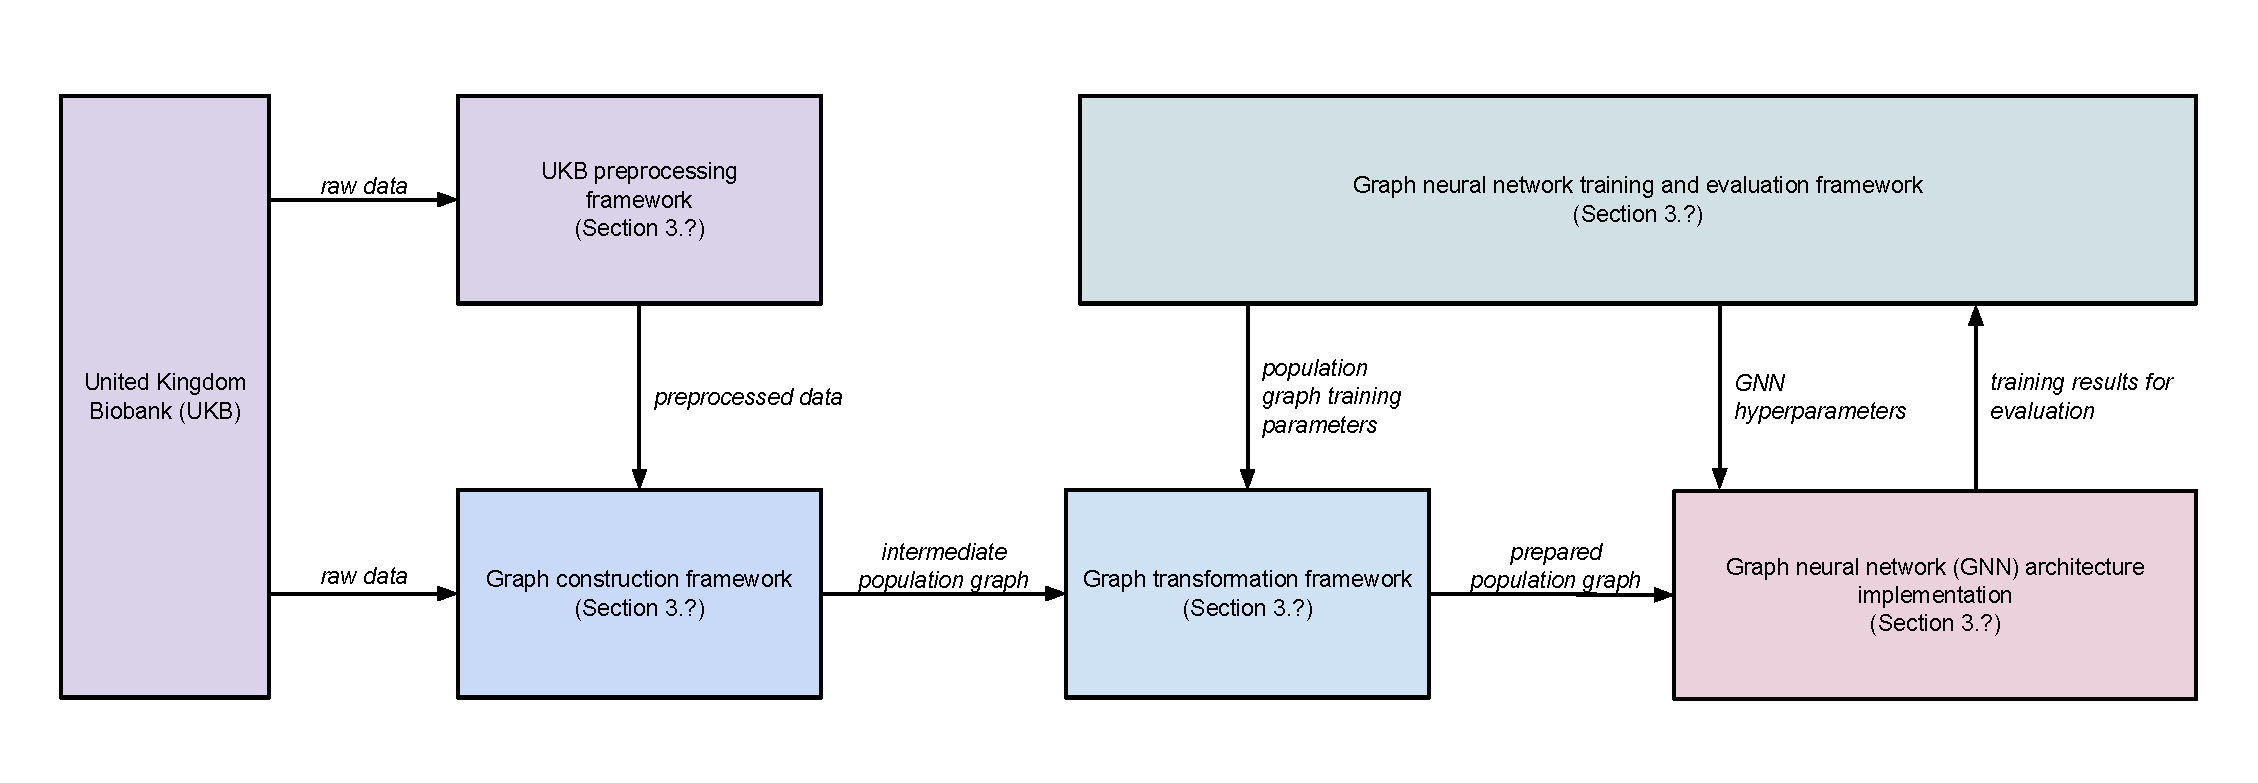
\includegraphics[width=\textwidth]{pipeline_overview.pdf}
    \caption{Overview of the key project components.}\label{pipeline-overview}
\end{figure}

This project can be divided into five key components (Figure~\ref{pipeline-overview}):
\begin{enumerate}
    \item Preparation of the United Kingdom Biobank (UKB) dataset;
    \item Intermediate population graph construction;
    \item Population graph transformation for training;
    \item Training on graph neural network architectures;
    \item Evaluation of the graph neural network performance.
\end{enumerate}

This chapter will explain in detail the steps behind each of the stages.

TODO fill the page (can make a bigger diagram!)

\newpage

\section{UKB preprocessing component}
\begin{figure}[]
    \centering
    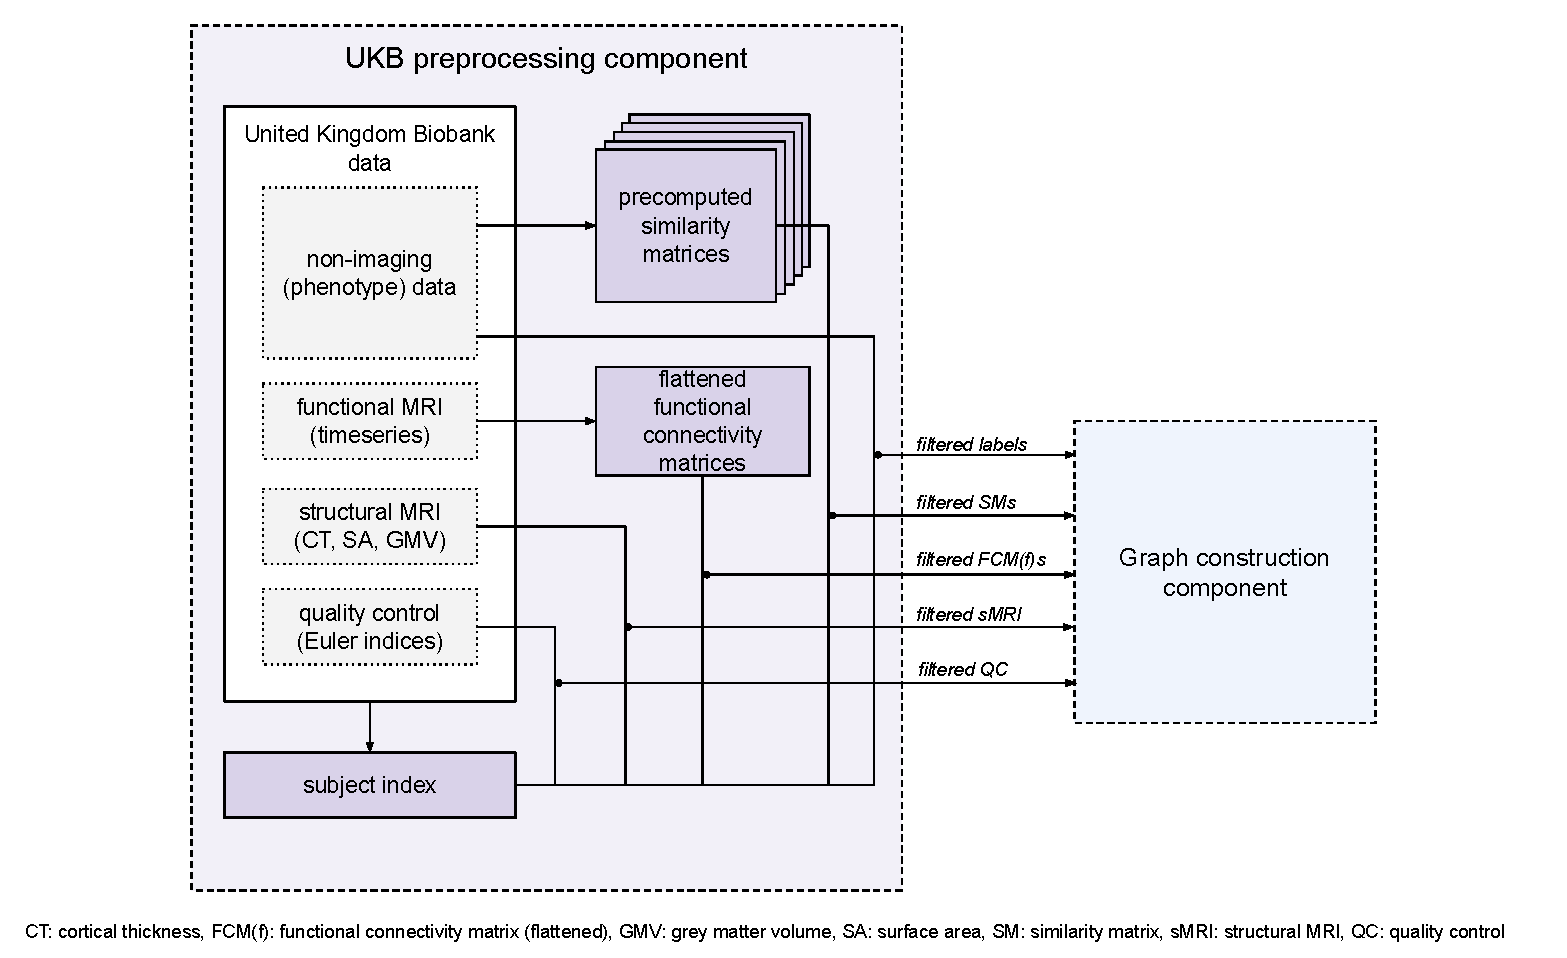
\includegraphics[width=\textwidth]{preprocessing_component.pdf}
    \caption{UKB preprocessing component.}\label{preprocessing-component}
\end{figure}

The main function of the UKB preprocessing component is to prepare the raw or partially preprocessed UKB data for population graph construction (Figure~\ref{preprocessing-component}). In particular, to improve the computational efficiency of most of the operations later in the pipeline, this component precomputes some of the data in the convenient form. This involves cleaning the dataset, precomputing similarity matrices and functional connectivity matrices.

\subsection{Cleaning the dataset}
While the United Kingdom Biobank is very well maintained and the data is nicely structured, the different modalities (functional MRI, structural MRI, phenotype data, Euler indices—as shown by different components in Figure~\ref{preprocessing-component}) were provided separately. The functional data contains scans for 17,550 patients, but 233 of them had missing data in other modalities (it was retracted from the biobank but the scans remained available). Three more patients have had corrupted brain scans (did not have a matching number of brain regions) which did not allow to create a meaningful functional connectivity matrix of the same dimension as all the others and were therefore discarded. The 17314 patients that had the data available for all modalities hve been collected into a \textit{subject index} (Figure). 
TODO Explain what does filtered data mean.

\subsection{Precomputing connectivity matrices}
The connectivity matrices involve computing the pairwise correlations of 376 time-series for every subject, a $O(N^2)$ computation for the dataset of  $N$ subjects. With 20 GB of raw timeseries data across 17,000 subjects, this introduces a high computational overhead (a few hours) if the matrices are computed on the fly as the graph is constructed. An additional inefficiency comes from the computation being repeated whenever a population graph that uses the functional data is constructed (which might be frequent when different graph parameterisations are explored). To avoid the inefficiency, the matrices are computed once for each subject, flattened and their lower triangles stored as NumPy arrays before the graph is constructed.

TODO \textit{could include the maths here?}

\subsection{Precomputing similarity matrices}
While the non-imaging modalities used for similarity computation are much smaller in file size, the computation of the similarity function is also pairwise. The $O(N^2)$ computation that involves pairwise comparison, addition and averaging of values for each non-imaging metric might take hours or even days for the full dataset to be processed, depending on the exact similarity definition. This computation is also repeated whenever a graph is constructed, since the similarities per non-imaging metric do not change over different graphs: the variation comes from different selections of metrics, their relative weighting, and similarity thresholds.

The similarity matrices have therefore been computed in advance. Unlike the functional connectivity data used directly as node features, the metric-wise similarities need to be looked up quickly when computing the score for a given similarity function, so the full matrix is stored.

TODO reference phenotype table

For the \texttt{ICD10} metric, the subjects were considered to be \texttt{ICD10}-similar whenever they had at least one shared mental health or nervous system diagnosis, while two patients without any mental health or nervous system diagnoses were \textit{not} considered to be similar, as this would create too many edges and make the model run out of memory. The computation can be vectorised: for the boolean \texttt{ICD10}-lookup matrix $\mathbf{F}_{\text{icd10}}$ with rows indexed by subjects and columns by relevant \texttt{ICD10} diagnoses, the pairwise similarity matrix $\mathbf{M}_{\text{icd10}}$ computation corresponds to 

\begin{equation}
    \mathbf{M}_{\text{icd10}} = \mathbf{1}\left[\mathbf{F}_{\text{icd10}}^{\ }\mathbf{F}_{\text{icd10}}^{\mathrm{T}} \geq 1\right]
\end{equation}

where the indicator function $\mathbf{1}[\cdot]$ is applied element-wise.

For the remaining metrics (e.g. years of full-time education, \texttt{FTE}) there is only one integer or floating-point value per subject, with values  compared for equality. The operation is vectorised by exploiting NumPy's broadcasting operation that copies rows and columns as necessary for the matrix dimensions to match: for the \texttt{FTE} lookup vector $\mathbf{f}_{\text{fte}}^{\mathrm{T}} \in \mathbb{R}^{N \times 1}$ and $\mathbf{F}_{\text{fte}} = [\mathbf{f}_{\text{fte}}^{\mathrm{T}} \cdots \mathbf{f}_{\text{fte}}^{\mathrm{T}}] \in \mathbb{R}^{N \times N}$, \texttt{FTE}-similarity matrix is defined as

\begin{equation}
    \mathbf{M}_{\text{fte}} = \mathbf{1}\left[\mathbf{F}_{\text{fte}}^{\ } = \mathbf{F}_{\text{fte}}^{\mathrm{T}} \right].
\end{equation}


% \[
% \begin{blockarray}{rccccc}
%  & b & c & d & e & f \\
% \begin{block}{r[ccccc]}
%   \text{UKB} & 1 & 1 & 1 & 1 & f \\
%   0 & 1 & 0 & 0 & 1 & g \\
%   0 & 0 & 1 & 0 & 1 & h \\
%   0 & 0 & 0 & 1 & 1 & i \\
%   0 & 0 & 0 & 0 & 1 & j \\
% \end{block}
% \end{blockarray}
%  \]










\section{Graph construction component}

\begin{figure}[h]
    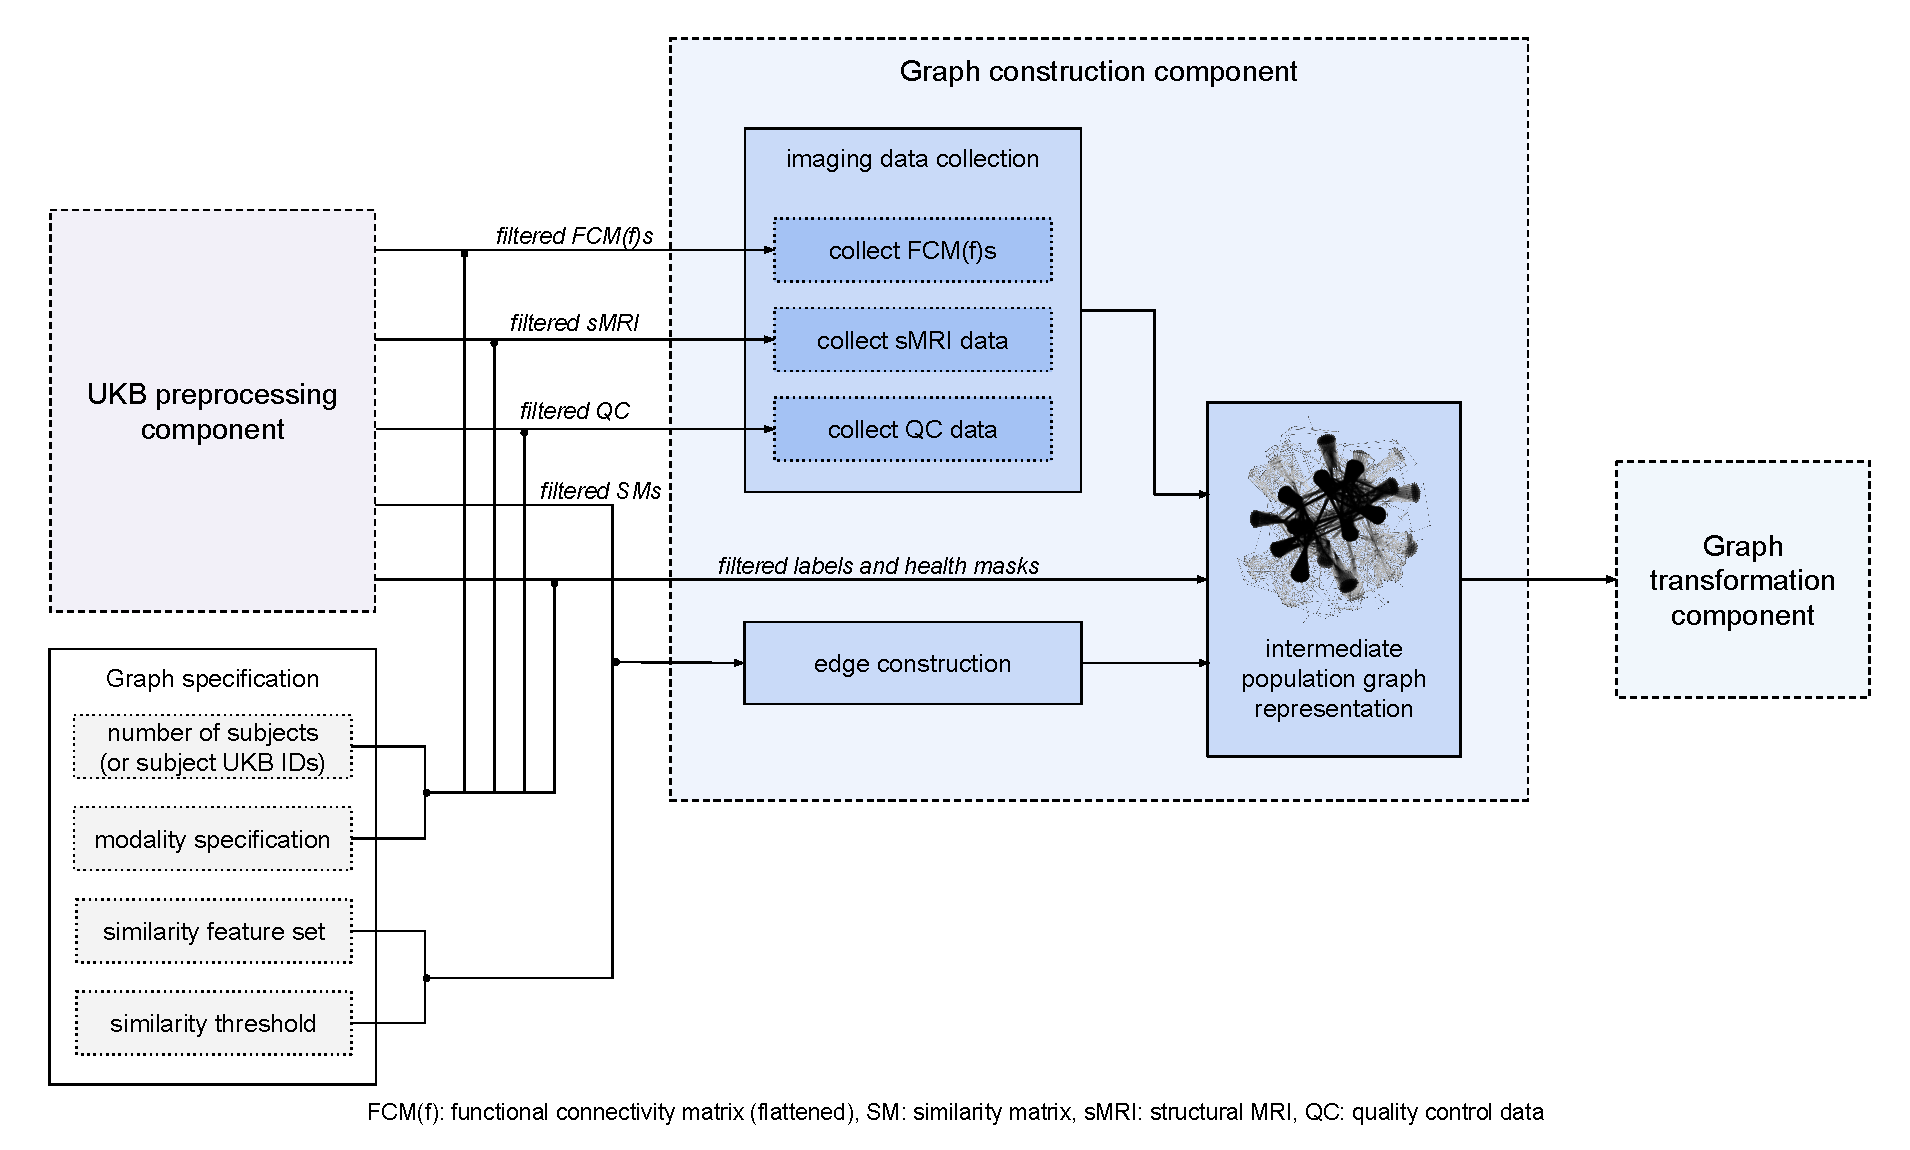
\includegraphics[width=\textwidth]{graph_construction_component.pdf}
    \caption{Graph construction component.}\label{graph-construction-component}
\end{figure}


\section{Graph transformation component}

\begin{figure}[h]
    \centering
    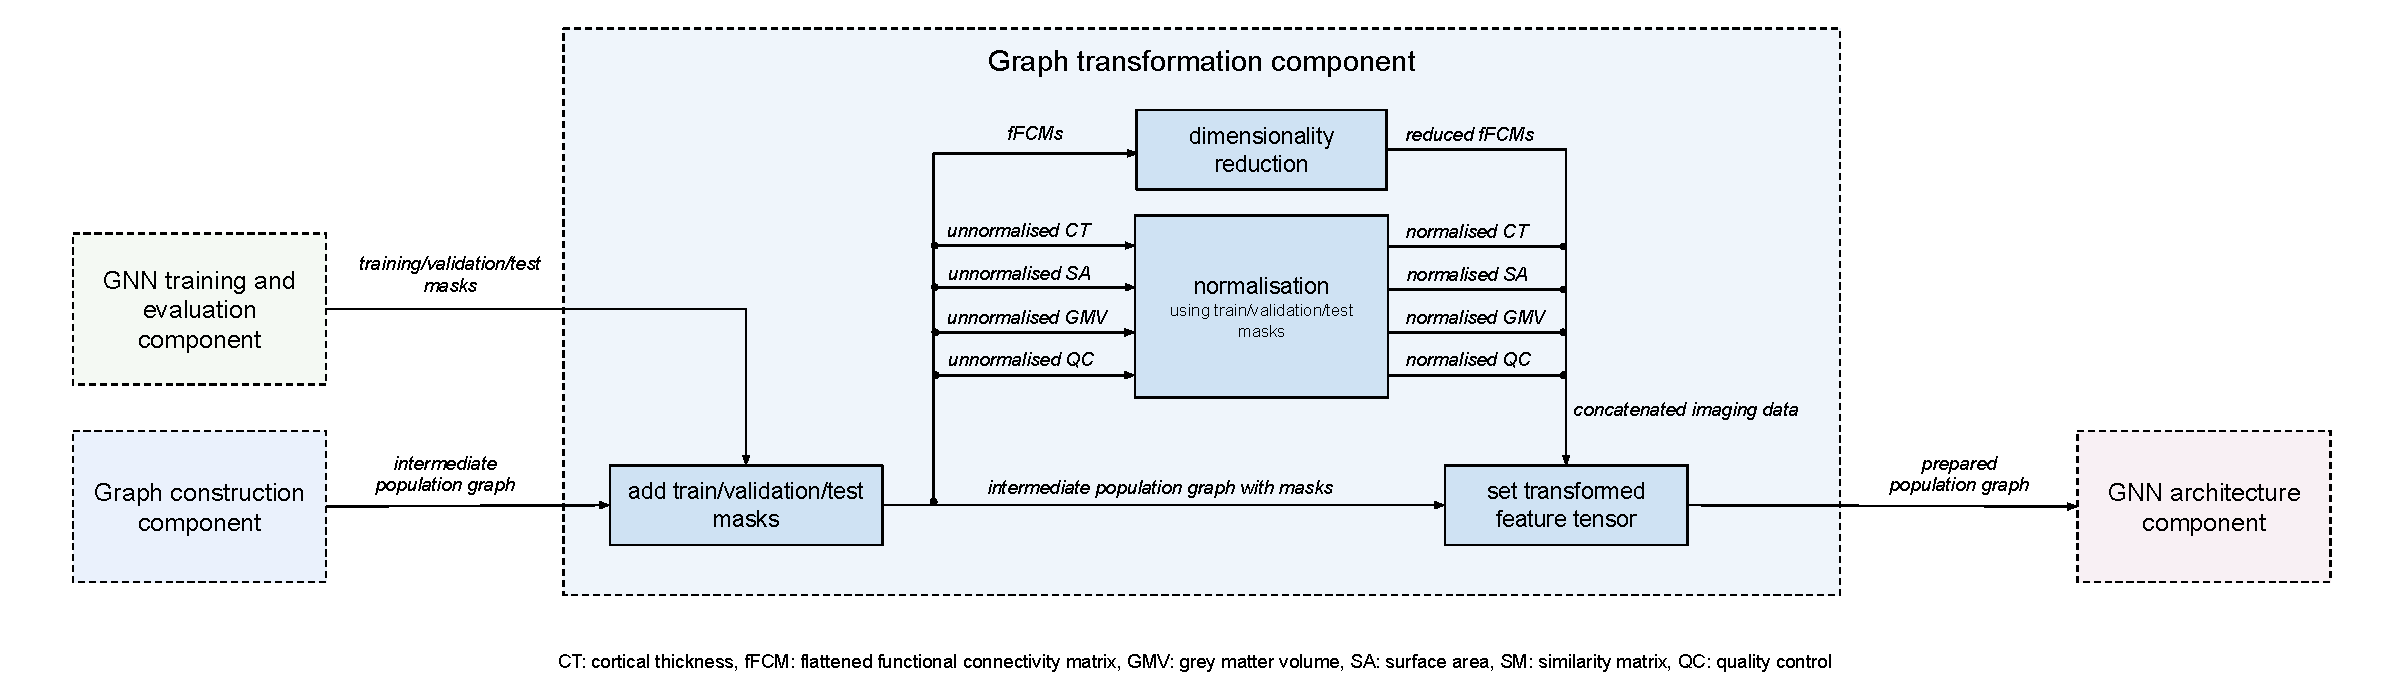
\includegraphics[width=\textwidth]{graph_transformation_component.pdf}
    \caption{Graph transformation component.}\label{graph-transformation-component}
\end{figure}

Describe how the graph intermediate representation is changed based on the training transformation parameters (training fold, train/validation/test set split). The intermediate graph is prepared for training by normalising the features based on the train subset, adding train/validation/test set masks to ignore subjects that should not be used for feedback in training, concatenating the multiple modalities into a single feature set.

Subject stratification, removing subjects with too few age occurrences because the data cannot be correctly stratified otherwise.


\section{Graph neural network component}
Description of architecture: number and size of layers etc.

Could have a diagram.


\section{Evaluation component}
The standard performance metrics $r$ and $r^2$ tracked and logged with training.

Describe the additional graph transformation stages which add noise to node features/edges.


\section{Repository overview}
% The repository overview should be around one page in length and should describe the high-level structure of the source code found in your source code Repository; ... could be implemented as a table with folders/file names and the functionality implemented in those files


\newpage




\subsection{UK Biobank subject selection}
Selecting the subset of subjects that has all data modalities available: some modalities (e.g. phenotypic data) were unavailable because the subjects retracted the permissions to use their data and were removed from the UK Biobank.

Three subjects with inconsistent functional MRI imaging data with some of the regions absent were discarded.


\subsection{Functional connectivity matrix precomputation}

\subsubsection{Dimensionality reduction for neural networks}
The full flattened functional connectivity matrix has over 75,000 features per patient, which, considering pairwise similarities and a large number of subjects, makes the graph (and the training on it) very large: the number of resulting training parameters runs out of memory even for small architectures.

The easiest solution mitigating this is running a PCA on the matrix, assuming that the first few principal components (how many?) would give a good representation of functional data features. Preliminary runs on small datasets of a few thousand subjects give similar performance.




\subsection{Intermediate graph representation}
Describe the resulting intermediate representation as graph construction pipeline is called with specific graph parameters.

Could here mention the \textit{extension} of having weighted edges where edge features would store raw similarity thresholds.

\subsubsection{Node features}
Stored raw because unclear how they should be normalised until the training parameters are set.

\subsubsection{Edge computation}




\subsection{Hyperparameter tuning}
Describe which hyperparameters were tuned using Bayesian optimisation strategy, early stopping, cross-validation etc.




